\documentclass{standalone}
\usepackage[edges]{forest}
\usetikzlibrary{shadows.blur}
\begin{document}
    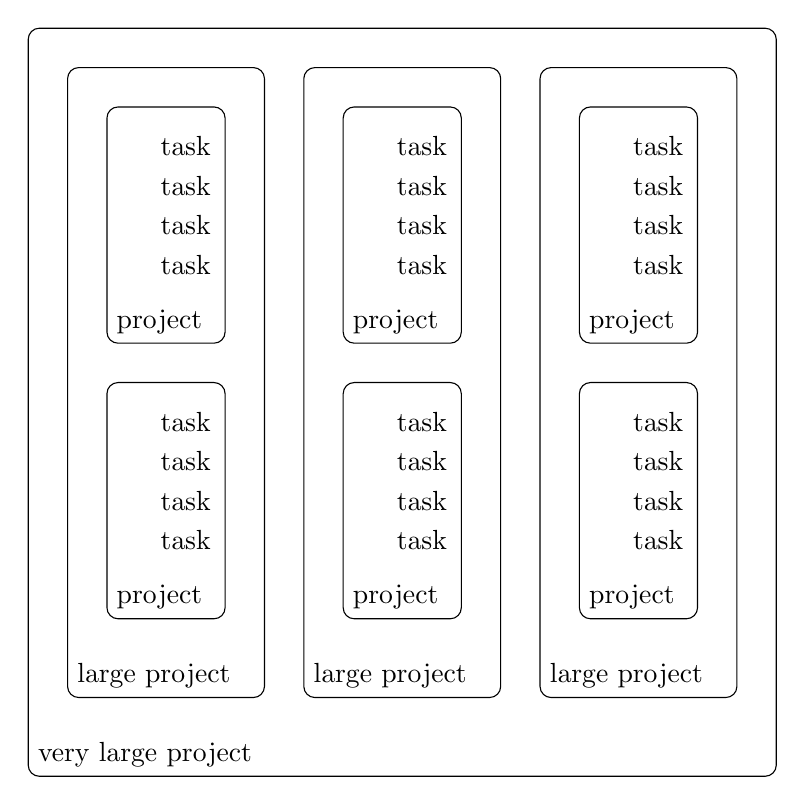
\begin{tikzpicture}
        \draw[rounded corners] (0,0) node[above right] {very large project} rectangle (9.5,9.5);
        
        \draw[rounded corners] (0.5,1) node[above right] {large project} rectangle (3,9);
        \draw[rounded corners] (3.5,1) node[above right] {large project} rectangle (6,9);
        \draw[rounded corners] (6.5,1) node[above right] {large project} rectangle (9,9);
        
        \draw[rounded corners] (1,2) node[above right] {project} rectangle (2.5,5);
        \draw[rounded corners] (4,2) node[above right] {project} rectangle (5.5,5);
        \draw[rounded corners] (7,2) node[above right] {project} rectangle (8.5,5);
        
        \draw[rounded corners] (1,5.5) node[above right] {project} rectangle (2.5,8.5);
        \draw[rounded corners] (4,5.5) node[above right] {project} rectangle (5.5,8.5);
        \draw[rounded corners] (7,5.5) node[above right] {project} rectangle (8.5,8.5);
        

        \foreach \i in {2,5,8}{
            \node at (\i,8) {task};
            \node at (\i,7.5) {task};
            \node at (\i,7) {task};
            \node at (\i,6.5) {task};
            \node at (\i,4.5) {task};
            \node at (\i,4) {task};
            \node at (\i,3.5) {task};
            \node at (\i,3) {task};
        }




    \end{tikzpicture}
    
\end{document}
